\section{Vehicle Actuated Programming in Vissim}
\label{vap}
VAP is an optional module for Vissim which enables direct programming of signal controllers. VAP is a simple, label-based (goto) language. The main feature is access to a library of functions, which manipulate the state of the signal controller. 

With VAP there is a graphical program, VISVAP, that allows the user to design a flowchart description of the controller logic, rather than writing it in VAP, as VISVAP can compile the flowchart into VAP. Figure \ref{fig:visvap_example} shows an example of a simple logic to control the lights at the ring 3 / Herlev Sygehus intersection.

\begin{figure}[!ht]
\begin{center}
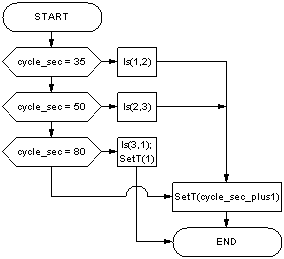
\includegraphics[scale=0.5]{visvap_example_herlev-sygehus.png} 
\end{center}
\caption{VISVAP flowchart description of simple fixed-time logic for Herlev Sygehus / ring 3}
\label{fig:visvap_example}
\end{figure}

The VAP program is called once for every simulation second. The starting label is START and the program proceeds as indicated by the arrows until the END label has been reached. Diamond boxes are logical tests where the right-going arrow indicates TRUE and down-going indicates FALSE. Square boxes contain expressions, in this case we use \verb|Is(<stage_from>,<stage_to>)| to switch between stages, when a certain portion of the current cycle time has passed. Below is the VAP code, which corresponds to the flowchart:

\begin{verbatim}
/* EXPRESSIONS */ 
            cycle_sec := T;
            cycle_sec_plus1 := cycle_sec + 1;

/* MAIN PROGRAM */ 

S00Z001:    IF cycle_sec = 35 THEN
S01Z001:      Is(1,2)
            ELSE
S00Z002:      IF cycle_sec = 50 THEN
S01Z002:        Is(2,3)
              ELSE
S00Z003:        IF cycle_sec = 80 THEN
S01Z003:          Is(3,1); SetT(1);
                  GOTO PROG_ENDE
                END
              END
            END;
S02Z004:    SetT(cycle_sec_plus1)
PROG_ENDE:    .
\end{verbatim}

VAP is unsuited for complex controller logic, such as ones involving predictions and optimization by iteration. This is due to the fact that VAP only has support for basic programming language constructs and the label-based nature of the language, which is detrimental to larger code bases see eg. the statement by Dijkstra \cite{nogoto}. As an example the above VAP code could be simplified into:

\begin{verbatim}
function UpdateController(cycle_second){
   switch(cycle_second){
   case 35: Interstage(1,2)
   case 50: Interstage(2,3)
   case 80: Interstage(3,1); Set_cycle_second(1); return
   case else:  /* do nothing */
   }
   Set_cycle_second(cycle_second + 1) /* update time */
}
\end{verbatim}

VAP is suitable, however, for implementation of DOGS due to its simple decision system as described in section \ref{dogs}. In this section I will describe how the DOGS logic was implementated in VAP.

\subsection*{Interstage Definitions - PUA}
Before we move on to DOGS in VAP it is fundamental to explain the \verb|Interstage| (abbr. \verb|Is|) concept.

An interstage is basically the lighting scheme to be used during stage transition. Usually, when switching from stage A to B the lights of A switch to amber and then red while B switch from red to red and amber and then green.

The amber light of A is a warning that a transition is in progress, the intersection should be cleared and no more entries should be made. To ensure right-of-way consistency during the transition, B will stay red until the moment A switches from amber to red. For all intersections discussed in this project, the amber period is 4 seconds.

The red and amber period of B indicates that attentive entry into the intersection is permitted. The red and amber period is 2 seconds for all intersections.

Thus a total stage transition will last 6 seconds. In Figure \ref{fig:lost_time_example} is an example of the interstage lost times for various number of stages and cycle times. Some stages - eg. a through, left and rightgoing stage followed by a left-only stage - will be \textit{compatible} ie. there is no pause during the transition thus the table is pessimistic. However it clearly shows that there is a tradeoff between lost time and cycle time - especially in complex, multistaged intersections.

\begin{figure}[!ht]
\begin{center}
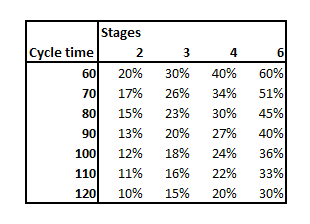
\includegraphics[scale=0.6]{interstage_lost_time.png} 
\end{center}
\caption{Interstage lost time in percent of cycle time for some combinations of cycle time and number of incompatible stages}
\label{fig:lost_time_example}
\end{figure}

In the above flowchart and code examples we start an interstage whenever we wish to move to the next stage.

The interstages are defined in Vissim by .PUA files. Below is an example of such a definition for Herlev Bygade. This intersection has two stages; stage A allowing traffic in either direction of the arterial and stage B for turn-ins from the minor road. 

\begin{verbatim}
$SIGNAL_GROUPS
A   1
B   2
$STAGES
Stage_1   A
red       B
Stage_2   B
red       A
$STARTING_STAGE
Stage_1
$INTERSTAGE1
Length [s]	 :   6
From Stage	 :   1
To Stage	   :   2
$    redend   grend
A    -127     0
B       6     127
$INTERSTAGE2
Length [s]	: 6
From Stage	: 2
To Stage	: 1
$    redend   grend
B    -127     0
A       6     127
$END
\end{verbatim}

In section \$STAGES it is defined that stage A should be green while B should is red and vice versa (they are not compatible). Here A and B refers to a space-separated list of signal groups from the \$SIGNAL\_GROUPS section.

For the interstage definitions, in INTERSTAGE1, we have redend for A to be -127, which means that A is green before the interstage, and grend (green end) is 0 meaning it should be red when the interstage has completed. For stage B, which is red before the interstage is run due to the \$STAGES definition, the redend (=green start) occurs 6 seconds into the interstage and grend set to 127 means that B should remain green after the interstage.

It is always up to the interstage designer to ensure that no right-of-way conflicts are present in the stage definitions. PTV supplies a support tool, which solves this issue, called CROSSIG though it was not employed in this project. CROSSIG is capable of generating .PUA files; in this project they were written manually, however.

\subsection{DOGS}
As VAP does not permit the writing of a program, which supervise all signal controllers at the same time, it was necessary to dedicate a signal controller as the master controller.

The master controller, which in Herlev is Herlev Hovedgade, runs the DOGS program and determines the current level by inspecting the northern- and southern detectors according to the specification outlined in section \ref{dogs}. In addition this controller also runs the master clock and the current DOGS level and cycle second is sent to all slave controllers every cycle second.

The slaves must listen for communication from the master controller and set the green time of the various stages according to the current dogs level and cycle second as received from the master.